\section{Intel KNL Architecture}
\label{src:knl}

Intel's popular Many Integrated Core (MIC) architectures are marked
under the name Xeon Phi and the second generation processors are
code
named Knights Landing (KNL). In
this paper, Intel KNL processors are used as an
example for emerging architectures with tiered memory systems. This
section provides a brief introduction to KNL
processor architecture.

Intel KNL offers at least 68 compute cores per chip with four
threads per core. %Apart from offering more than 2 TF double precision
%floating point performance, each KNL core supports two 512-bit vector
%units and AVX-512 SIMD intructions.
The 68 compute cores are organized
in 34 tiles with each tile having 2 compute cores.% and a shared 1MB
%L2 cache.
These 34 tiles are placed in a 2D mesh and connected through
an on-chip interconnect. In addition to traditional
DDR\footnote{Intel KNL supports double data rate fourth-generation
(DDR4)
synchronous dynamic random-access memory.}, KNL offers an on-package
high bandwidth memory
technology called Multi-Channel DRAM (MCDRAM). It offers high
bandwidth up to 4X more than DDR, but with limited capacity (up to
16GB) when compared to DDR (up to 384GB).
%MCDRAM can be configured as a direct mapped L3 cache layer or as a
%distinct NUMA node. Configuring the MCDRAM as an L3 cache layer is a
%convenient way to port existing applications on to KNL based systems.
%However, configuring the MCDRAM as a distinct NUMA node and re-designing
%an application to fully take advantage of the high bandwidth offered
%by the MCDRAM can improve the performance of memory bandwidth bound
%applications.

\begin{figure}[!h]
    \vspace{-35pt}
    \hspace*{5mm}
    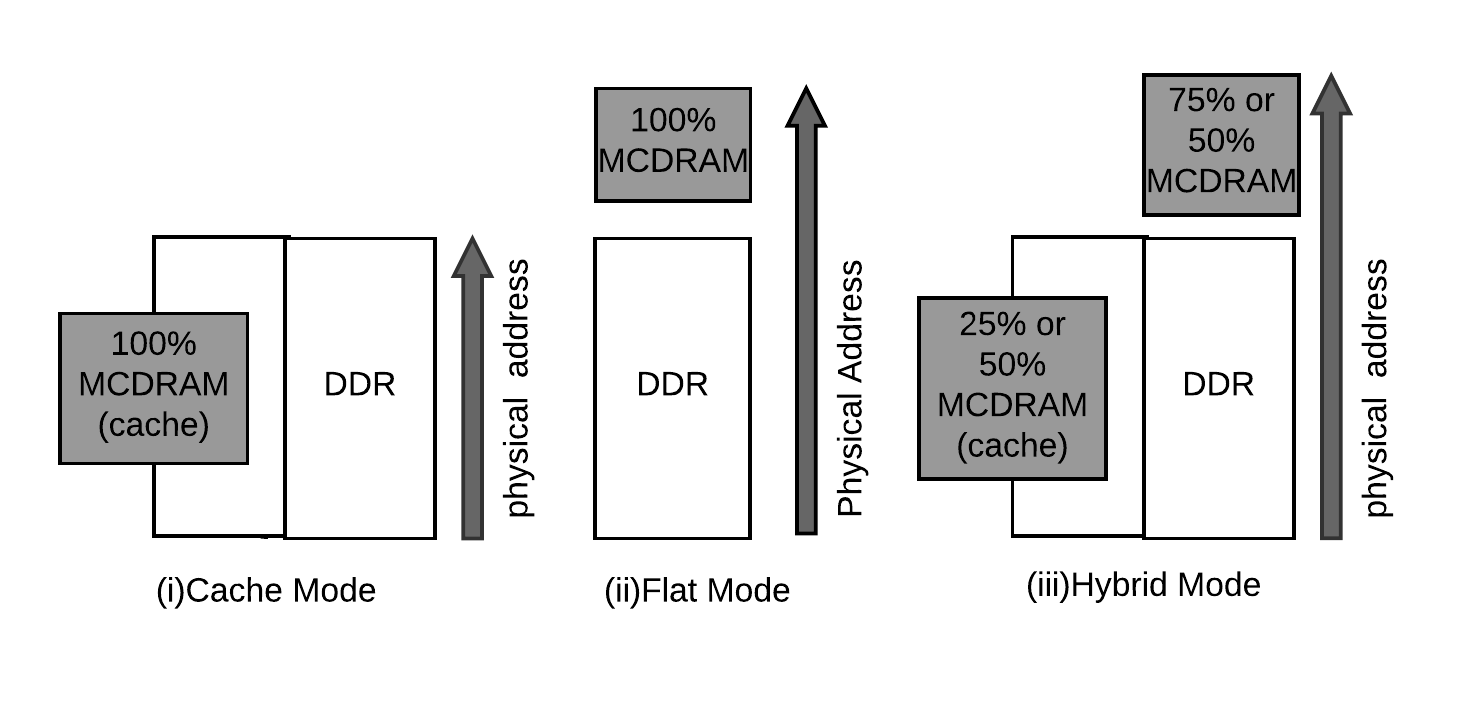
\includegraphics[scale=0.20]{image/mem-mode.png}
    \vspace{-25pt}
    \caption{Intel KNL Memory Configuration Modes}
    \vspace{-25pt}
    \label{fig:memmode}
\end{figure}

\subsection{Memory Modes}
\label{src:knl/config}
As shown in Fig.~\ref{fig:memmode}, MCDRAM can be configured in the
following modes.
\begin{itemize}
    \item \textbf{Cache mode} - in Cache mode
    MCDRAM acts as a last-level cache and it is completely used to
    cache the DDR data. %It is a convenient way to port existing
    %applications on to KNL based systems;
    \item \textbf{Flat mode} - in Flat mode the complete
    MCDRAM is available as an addressable memory and share the
    physical address space with DDR. With respect to Non Uniform
    Memory Access (NUMA), it is exposed as a separate NUMA node
    without cores.% and DDR is exposed as another NUMA node with
    %all the cores.
    %Configuring MCDRAM as a distinct NUMA node and
    %re-designing an application to fully take advantage of the high
    %bandwidth offered by the MCDRAM can improve the performance of
    %memory bandwidth bound applications; and
    \item \textbf{Hybrid mode} - as the name suggests, in
    Hybrid mode a portion of MCDRAM is configured as addressable
    memory and the rest as cache.
\end{itemize}

\subsection{NUMA Cluster Modes}
\label{src:knl/cluster}
As specified previously, the 68 compute cores are arranged in a 2D
mesh and connected using on-chip interconnect. With NUMA some memory
on the node has different latency or bandwidth to the core. %Based on
%clustering,
There are two important types of NUMA modes: Quadrant and
Sub-NUMA Clustering (SNC).

In quadrant mode the chip is divided into four different quadrants, but
it is exposed as a single NUMA domain. In SNC mode each quadrant is
available as a separate NUMA domain. Based on the number of quadrants
it is further divided into SNC2 and SNC4 modes.
